O objetivo deste relatório é fornecer bases analíticas com evidências empíricas como um de vários insumos para o desenvolvimento de políticas de Educação Profissional e Tecnológica (EPT) no contexto do PROPAG. A \href{https://datanalytics.worldbank.org/content/6604f317-d487-436a-b6b6-792369b341f0}{Plataforma Analítica Juros por Educação do BM--FGV} organiza estas análises em cinco dimensões fundamentais: (A) contexto demográfico e populacional; (B) cenários financeiros e simulações do PROPAG; (C) oferta atual e projetada de EPT; (D) demanda por formação técnica com base no desenvolvimento econômico regional; e (E) análise integrada entre oferta e demanda. A ferramenta permite ao usuário explorar dados detalhados de sua unidade federativa, realizar comparações entre estados e regiões, e simular diferentes cenários de adesão ao programa, oferecendo assim um conjunto robusto de informações para a definição de políticas sobre a expansão da EPT como fator importante para aumentar a produtividade do trabalhador no Brasil.

\begin{center}
	\textbf{\textcolor{orange}{Plataforma Interativo na Internet:}}\\
	\href{https://datanalytics.worldbank.org/content/6604f317-d487-436a-b6b6-792369b341f0}{https://datanalytics.worldbank.org/Plataforma-Interativo-PROPAG}
\end{center}

\section{Navegação da Plataforma}

A plataforma está estruturada em \textbf{múltiplas abas temáticas}, cada uma voltada a um aspecto crítico para a tomada de decisão. A interface principal, ilustrada na Figura~\ref{fig:intro_page}, apresenta todas as dimensões de análise organizadas de forma intuitiva.

\begin{figure}[htbp]
	\centering
	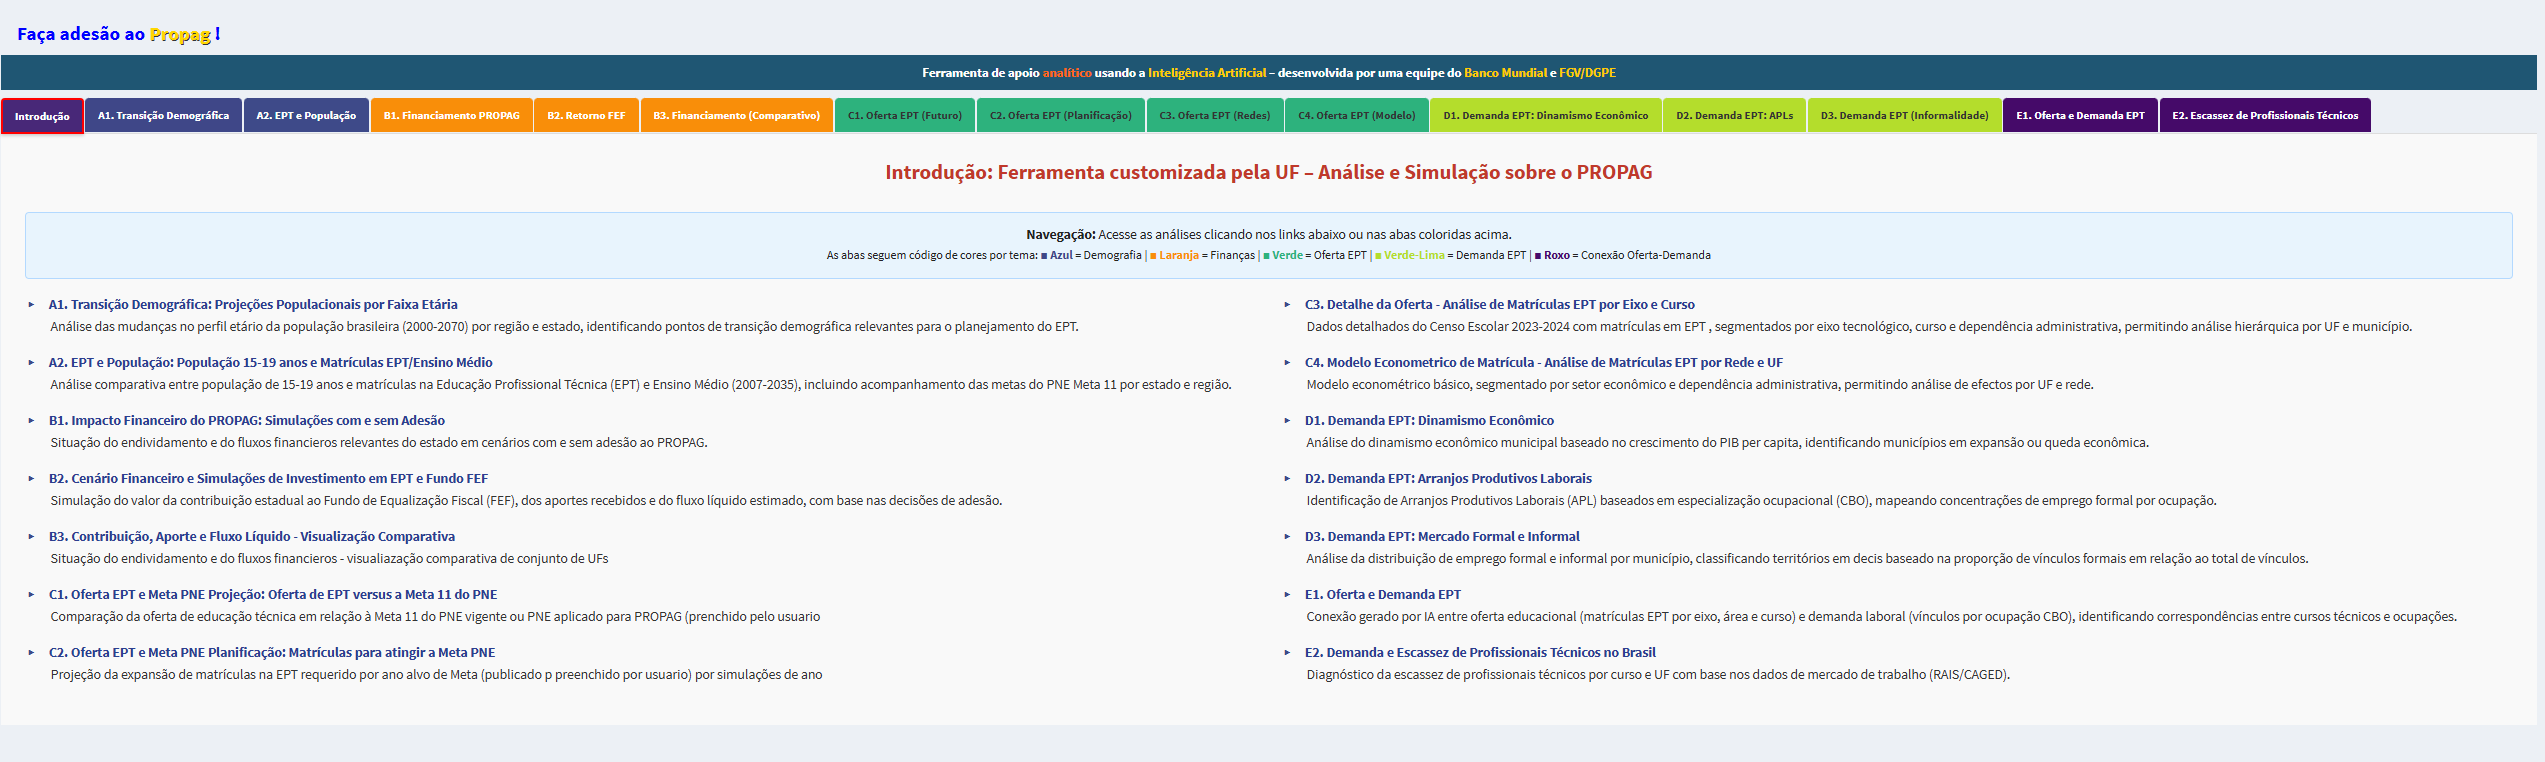
\includegraphics[width=\textwidth]{images/1a_IntroPage.png}
	\caption{Página inicial da Plataforma Analítica Juros por Educação - Interface de navegação com links diretos para todas as análises disponíveis}
	\label{fig:intro_page}
\end{figure}


As análises disponíveis na plataforma incluem:

\begin{itemize}
	\item \textbf{Cenário Financeiro e Simulações:} estima o espaço fiscal gerado pela adesão ao PROPAG e os aportes mínimos em EPT e no Fundo de Equalização Fiscal (FEF).
	
	\item \textbf{Impacto Financeiro com e sem Adesão:} compara a trajetória da dívida estadual em diferentes cenários.
	
	\item \textbf{Retorno do FEF por Opções:} mostra como as escolhas de opção de adesão afetam o saldo líquido estadual.
	
	\item \textbf{Projeções de Oferta e Meta 11 do PNE:} avalia a situação da matrícula em EPT em relação à meta nacional de triplicar o acesso.
	
	\item \textbf{Expansão de Matrículas e Novo PNE (2025--2035):} explora cenários para a próxima década de políticas educacionais.
	
	\item \textbf{Demanda e Escassez de Profissionais Técnicos:} cruza dados do mercado de trabalho (RAIS/CAGED) com a oferta de EPT para mapear gargalos regionais.
\end{itemize}

Além disso, a plataforma inclui \textbf{módulos demográficos} que permitem ao gestor compreender como a dinâmica etária afeta a demanda futura por educação, saúde e serviços sociais.


Com isso, a \textbf{Plataforma Analítica Juros por Educação do BM--FGV} funciona como um verdadeiro \textit{laboratório de simulação e análise}: o administrador estadual pode visualizar a situação do seu estado, comparar cenários de adesão ou não adesão ao PROPAG e planejar a aplicação dos recursos de forma estratégica, alinhando sustentabilidade fiscal, expansão da EPT e enfrentamento dos desafios demográficos.

A partir da página inicial, os usuários podem:
\begin{itemize}
	\item Navegar diretamente para qualquer análise clicando nas abas superiores coloridas
	\item Utilizar os links rápidos na página de introdução para acessar análises específicas
	\item Visualizar a organização temática completa da ferramenta
\end{itemize}

\vspace{1cm}
